\documentclass[conference]{IEEEtran}
\IEEEoverridecommandlockouts
% The preceding line is only needed to identify funding in the first footnote. If that is unneeded, please comment it out.
\usepackage{cite}
\usepackage{amsmath,amssymb,amsfonts}
\usepackage{algorithmic}
\usepackage{graphicx}
\usepackage{subcaption}


\usepackage{textcomp}
\usepackage{xcolor}
\def\BibTeX{{\rm B\kern-.05em{\sc i\kern-.025em b}\kern-.08em
    T\kern-.1667em\lower.7ex\hbox{E}\kern-.125emX}}
    
    
\graphicspath{ {./imgs/} }
    
\begin{document}

\title{Orange Detection Algorithm}

\author{\IEEEauthorblockN{Marshall Asch}
\IEEEauthorblockA{\textit{University of Guelph}\\
Guelph, Canada \\
masch@uoguelph.ca}
\and
\IEEEauthorblockN{Grant Douglas}
\IEEEauthorblockA{\textit{University of Guelph}\\
Guelph, Canada \\
gdouglas@uoguelph.ca}
}

\maketitle

\begin{abstract}
This document is a model and instructions for \LaTeX.
This and the IEEEtran.cls file define the components of your paper [title, text, heads, etc.]. *CRITICAL: Do Not Use Symbols, Special Characters, Footnotes, 
or Math in Paper Title or Abstract.
\end{abstract}

\begin{IEEEkeywords}
Image Processing, Fruit, Applied image colour segmentation, Automated counting
\end{IEEEkeywords}

\section{Introduction}

Counting and identifying the number of ripe fruits is important to automate harvesting fruits when they are ripe and to identify how many ripe fruits there are on a tree.

\section{Ease of Use}

\subsection{How we Selected the threshhold vales}


\section{Algorithms}

based off of this \cite{payne_estimation_2013}



\subsection{Values} \label{values}


\begin{figure*}[htbp]
\centerline{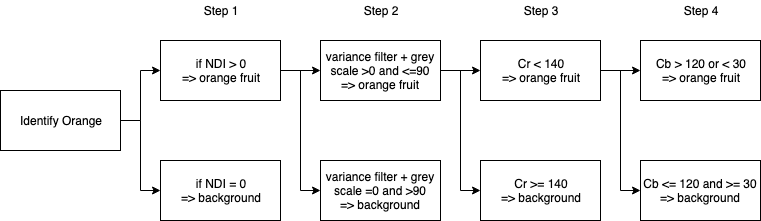
\includegraphics[width=\textwidth]{algo_stages}}
\caption{Outline of the proccess of the stages of the algorithm}
\label{fig}
\end{figure*}

\subsection{Stages}



\subsubsection{Step 1}
Run NDI 

\subsubsection{Step 2}
In the RGB colour space run a mean filter.

\subsubsection{Step 3}
convert the image to the YCrCb colour space.

run a threshold on the Cr values. how the threshold is discusses in sec. \ref{values}. 


\subsubsection{Step 4}

run a threshold on the Cb values. how the threshold is discusses in sec. \ref{values}. 

\subsubsection{Step 5}

Then do a bit-wise and to create a mask

\begin{equation}
pixel_{final}=pixel_{NDI} \land pixel_{mean} \land pixel_{Cr} \land pixel_{Cb} 
\end{equation}

\subsubsection{Step 6}
Do a circle count  on the mask image




\section{Results}

\begin{figure*}
  \begin{subfigure}{.33\linewidth}
 	 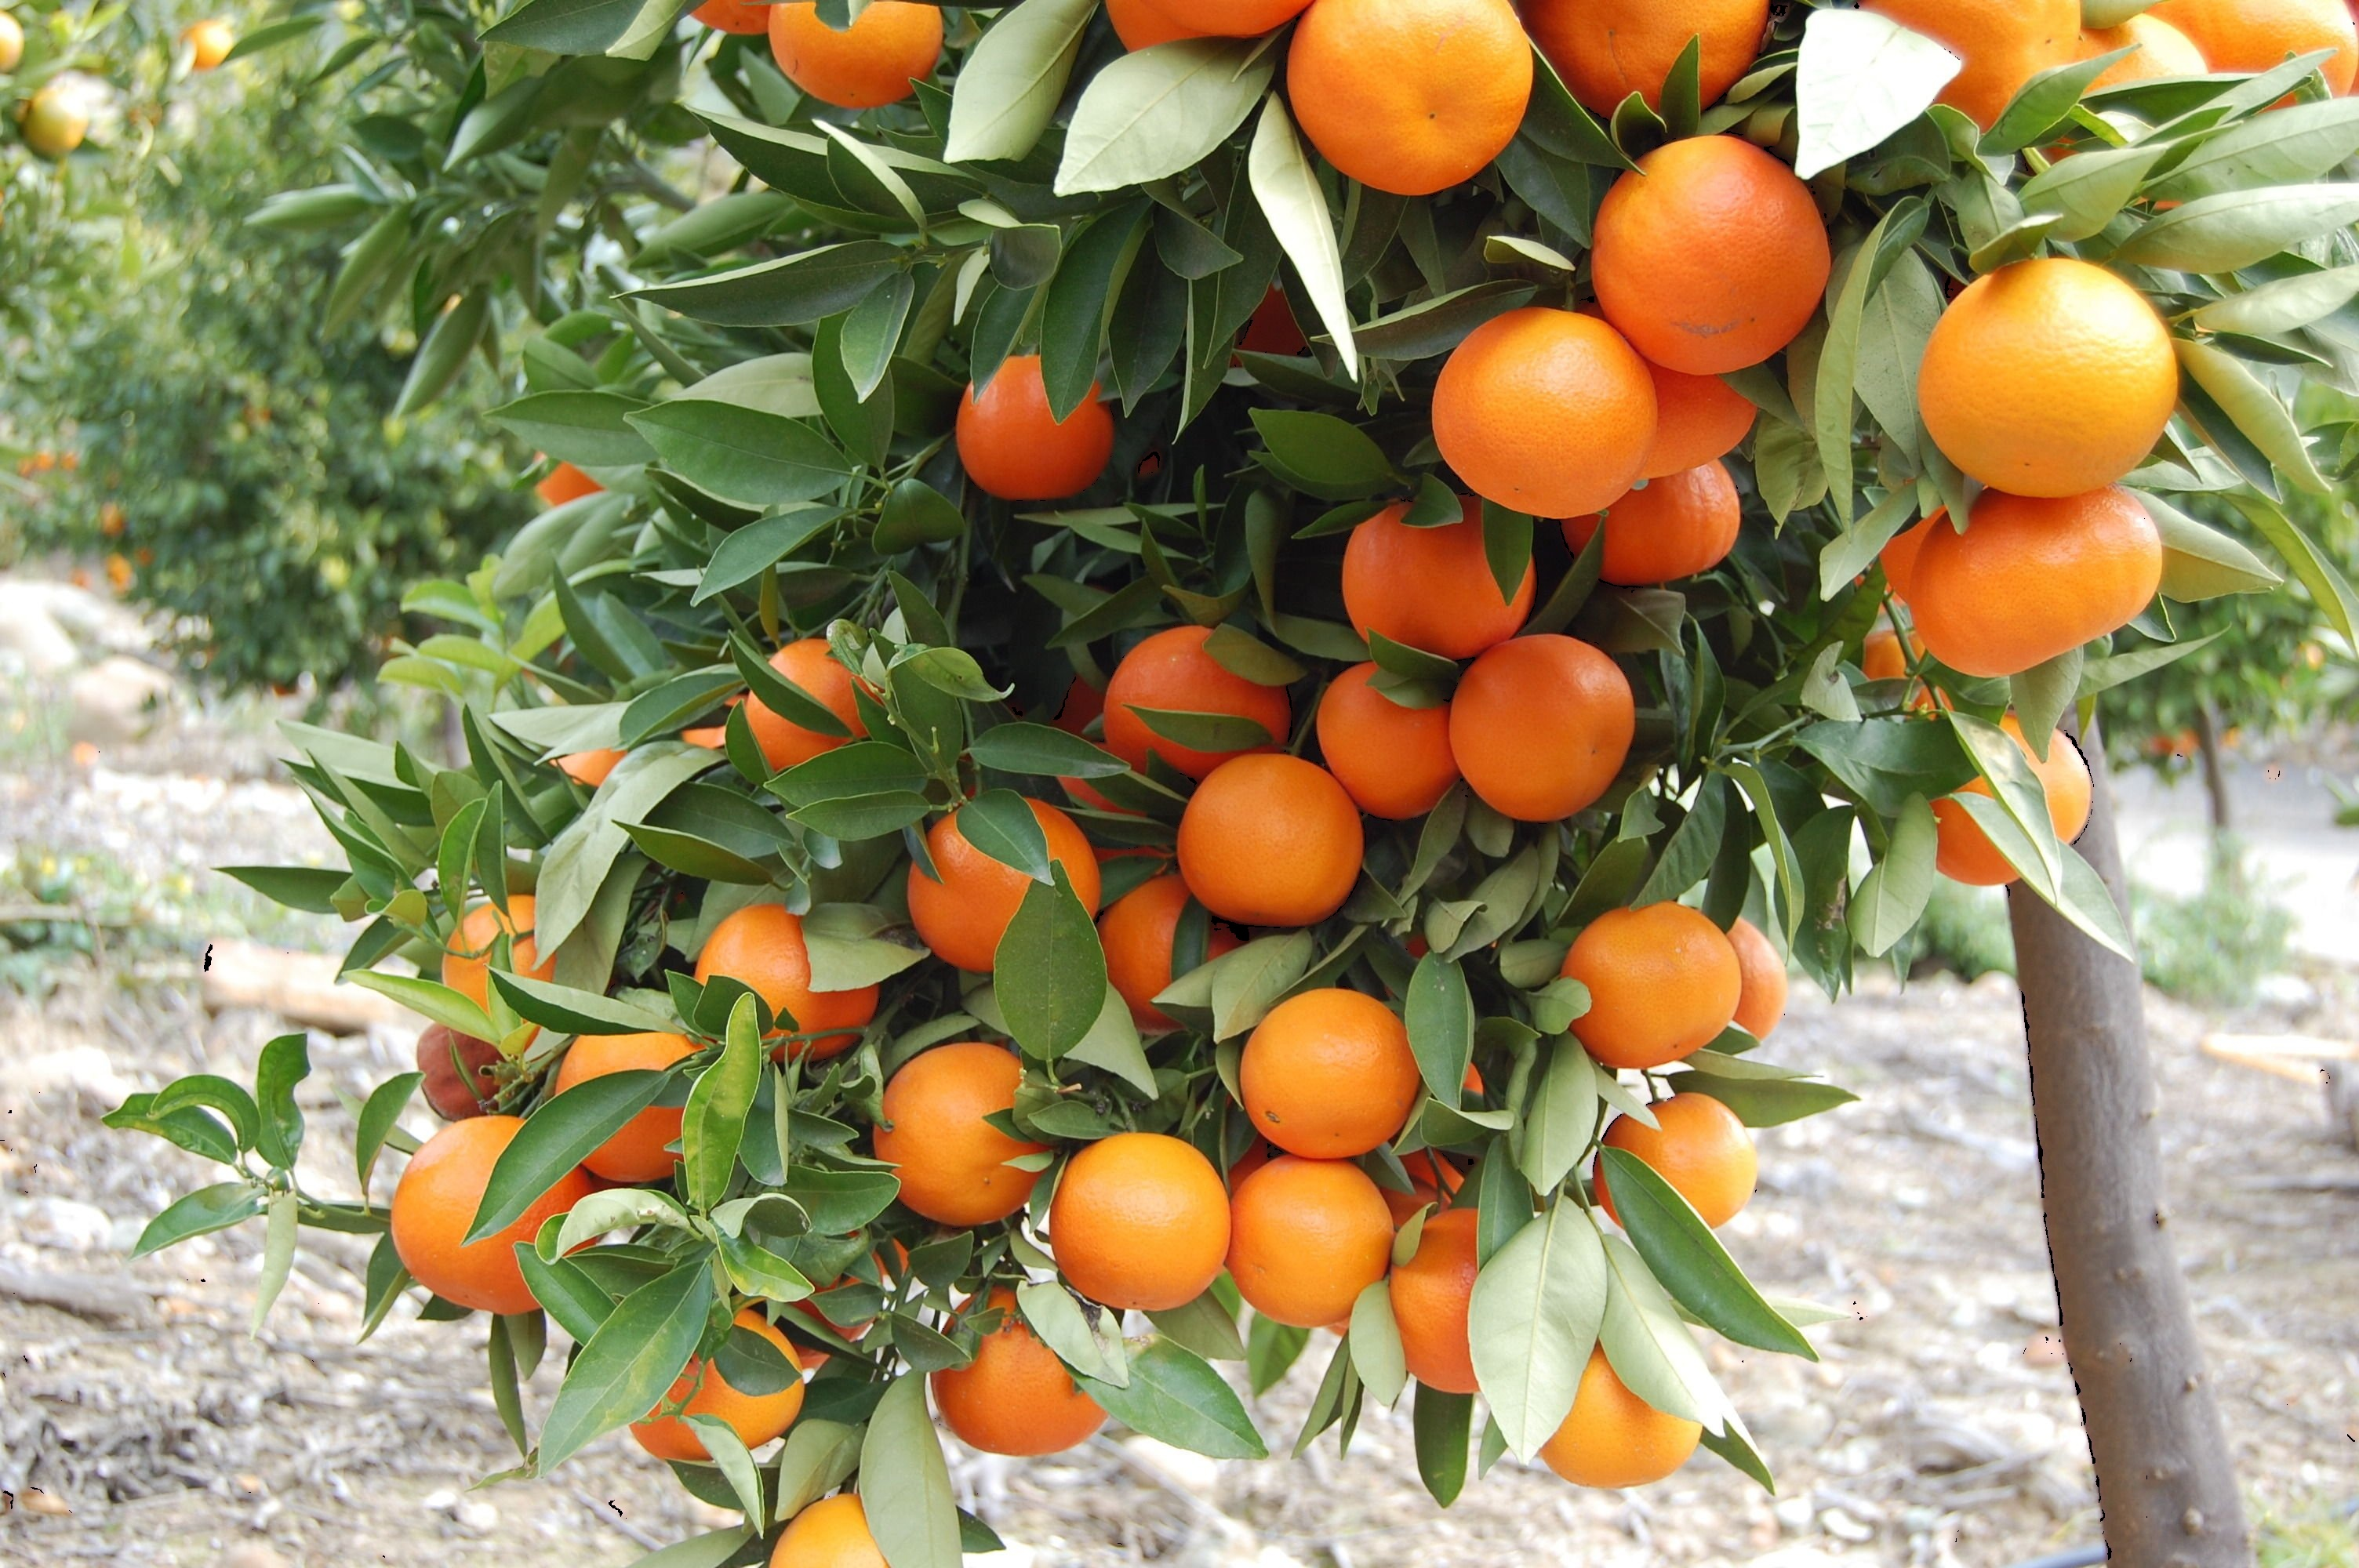
\includegraphics[width=\linewidth]{citrus1/citrus1_orig.jpg}\hfill
	 \caption{Origonal}
  \end{subfigure}
  \begin{subfigure}{.33\linewidth}
  	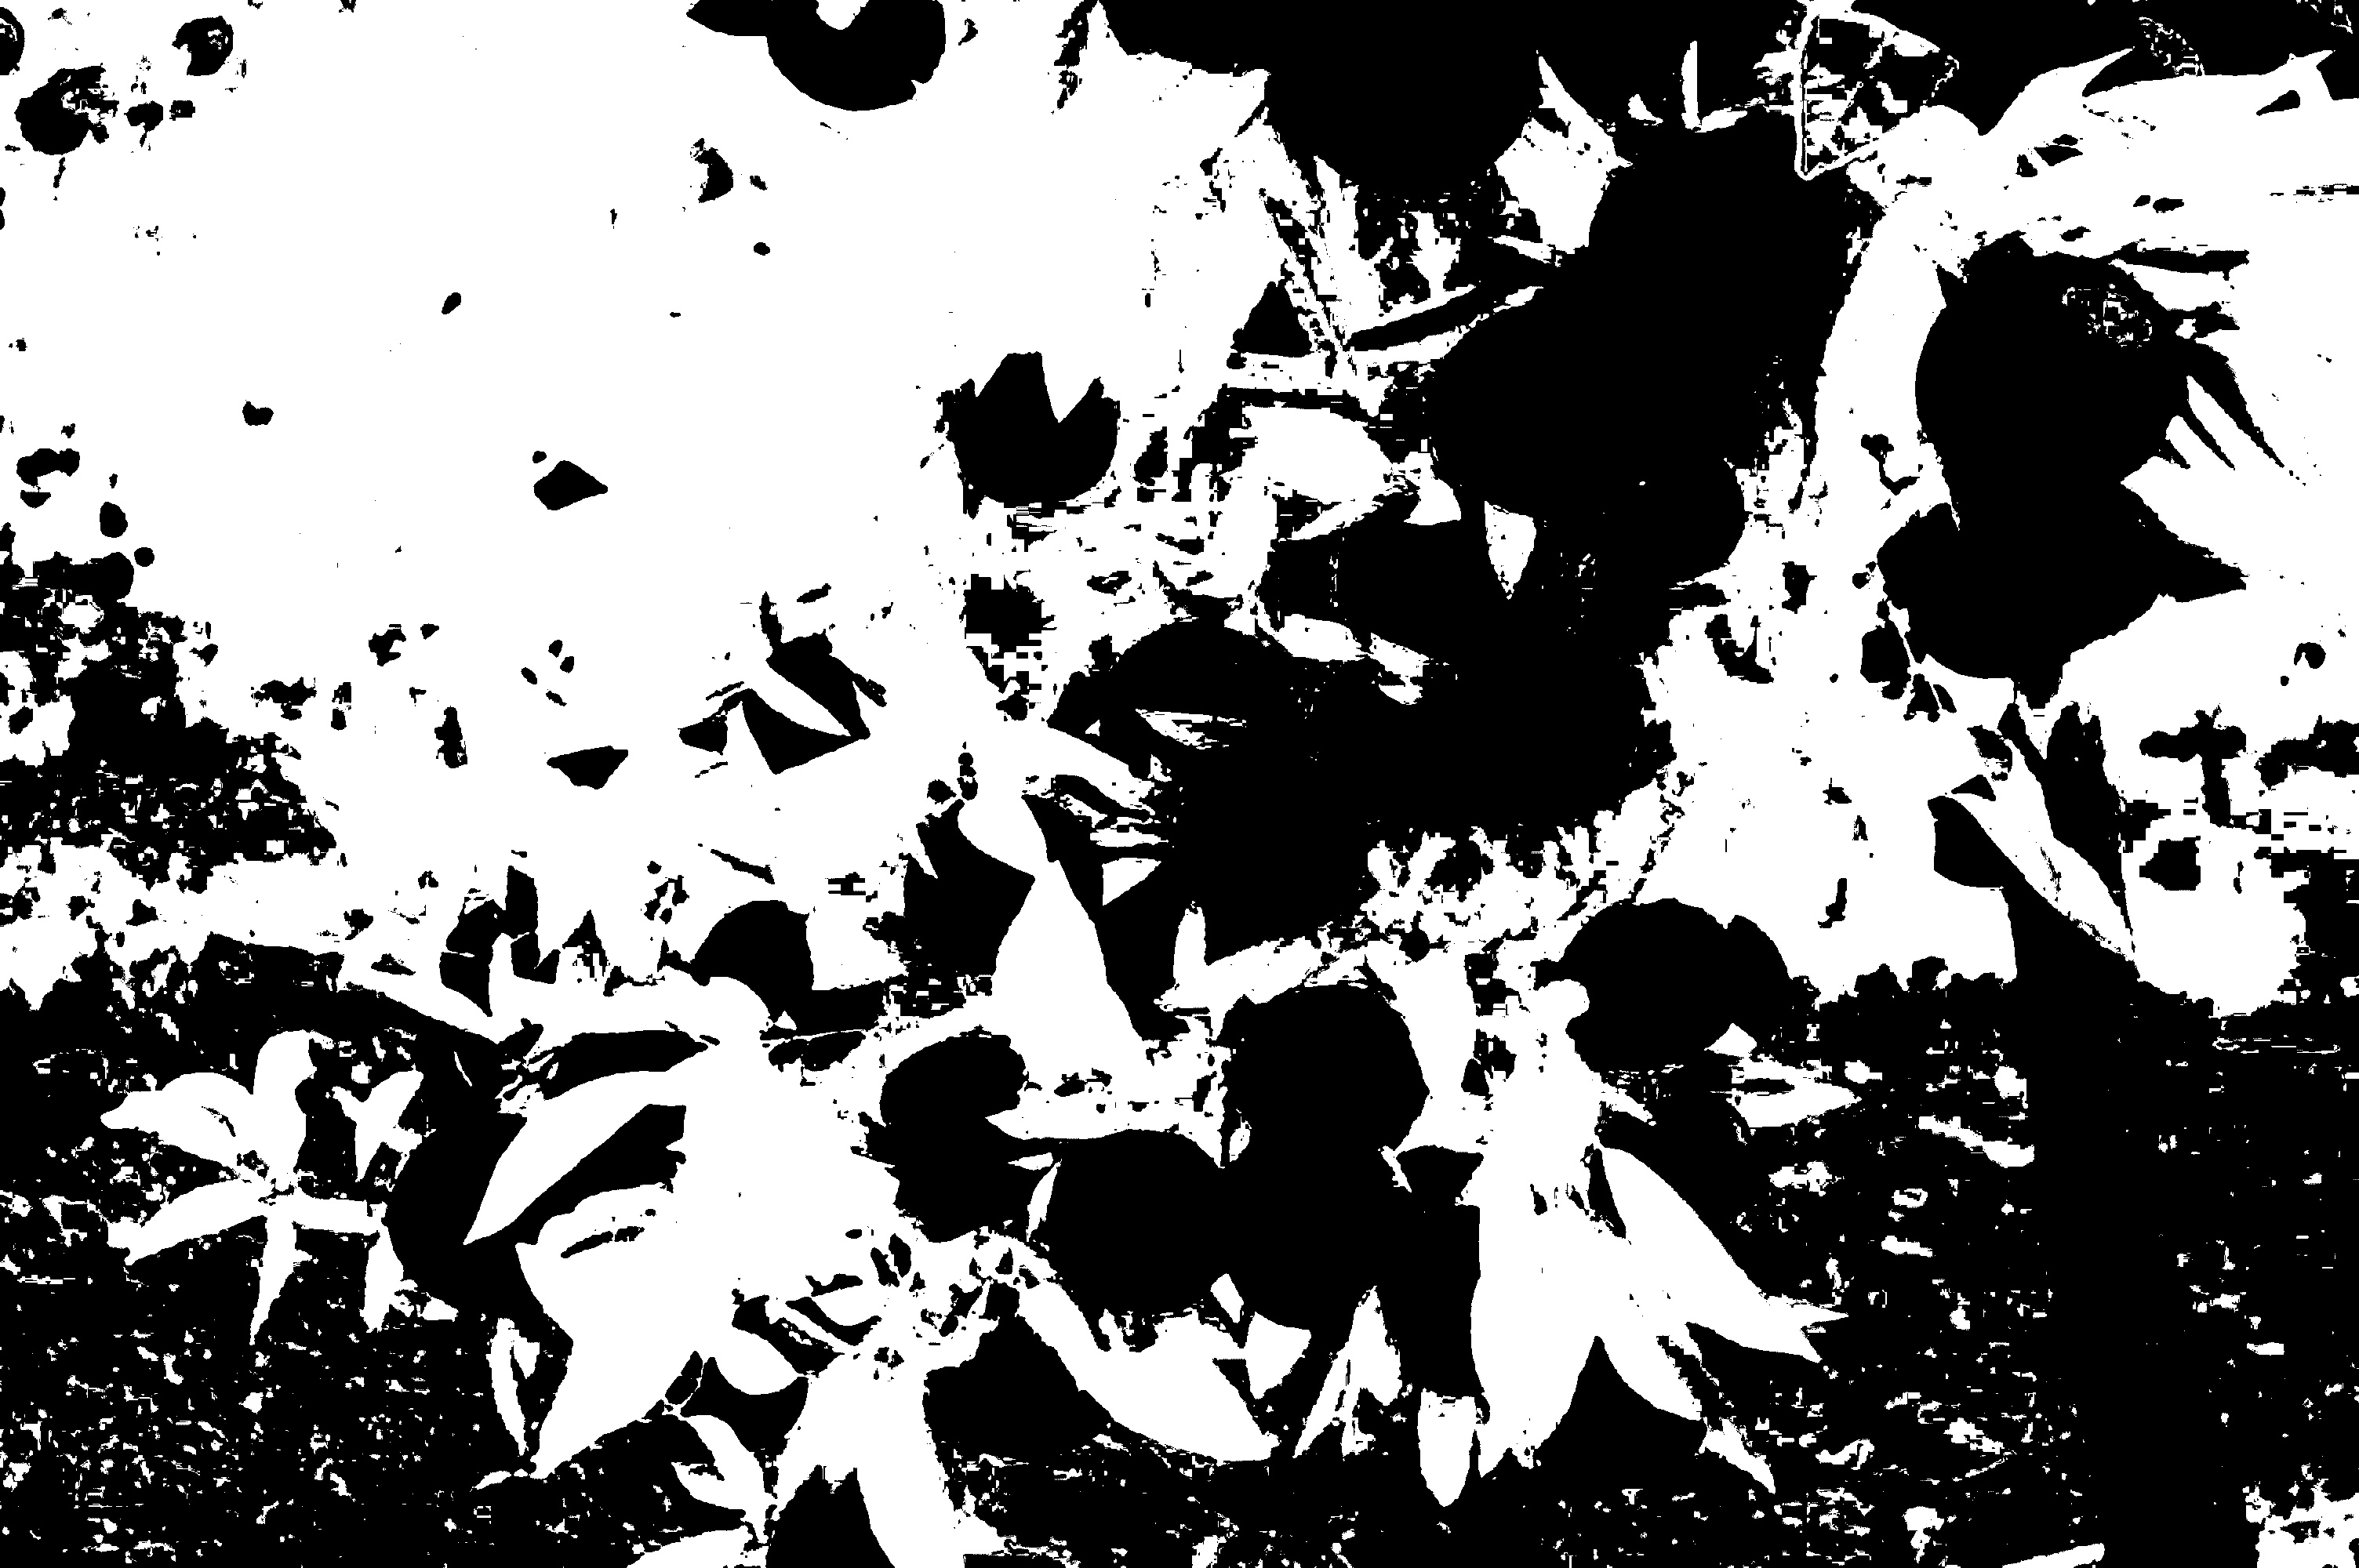
\includegraphics[width=\linewidth]{citrus1/citrus1_NDI.jpg}\hfill
   	\caption{Result of step 1}
  \end{subfigure}
  \begin{subfigure}{.33\linewidth}
  	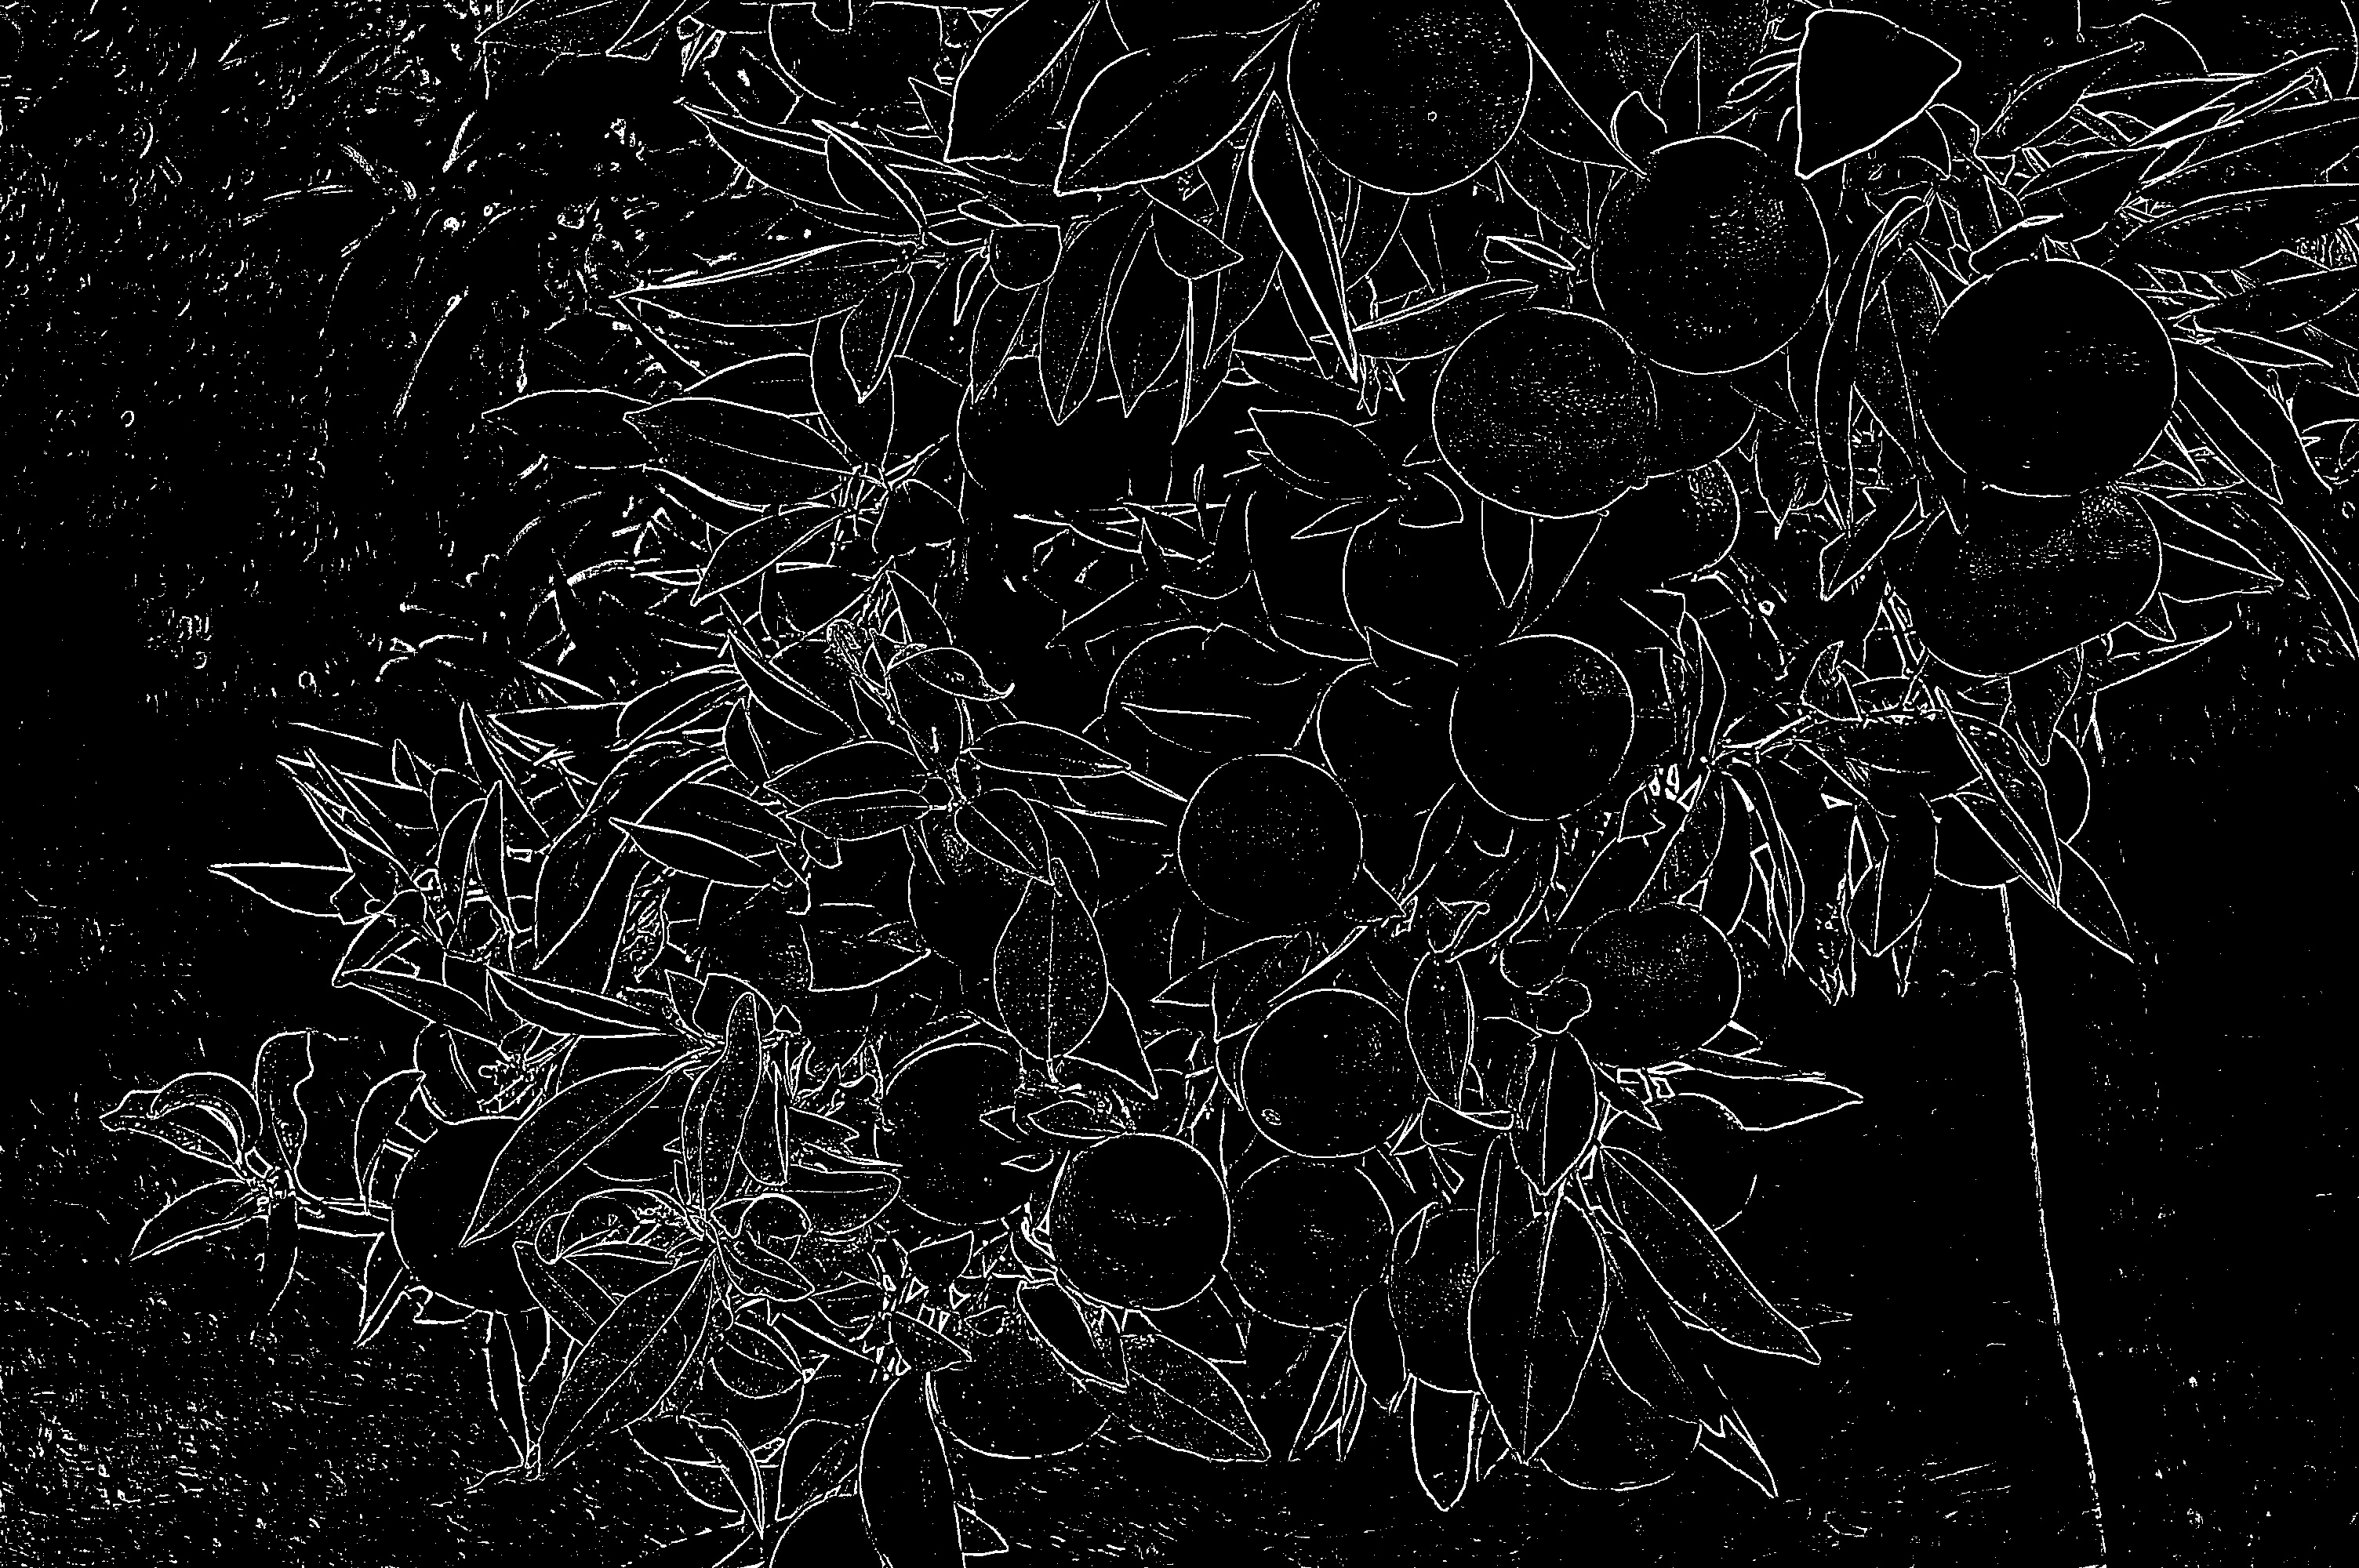
\includegraphics[width=\linewidth]{citrus1/citrus1_mean.jpg}
  	\caption{Result of step 2}
  \end{subfigure}\par\medskip
  
  \begin{subfigure}{.33\linewidth}
  	
\includegraphics[width=\linewidth]{citrus1/citrus1_cr.jpg}\hfill
     	\caption{Result of step 3}
  \end{subfigure}
  \begin{subfigure}{.33\linewidth}
  	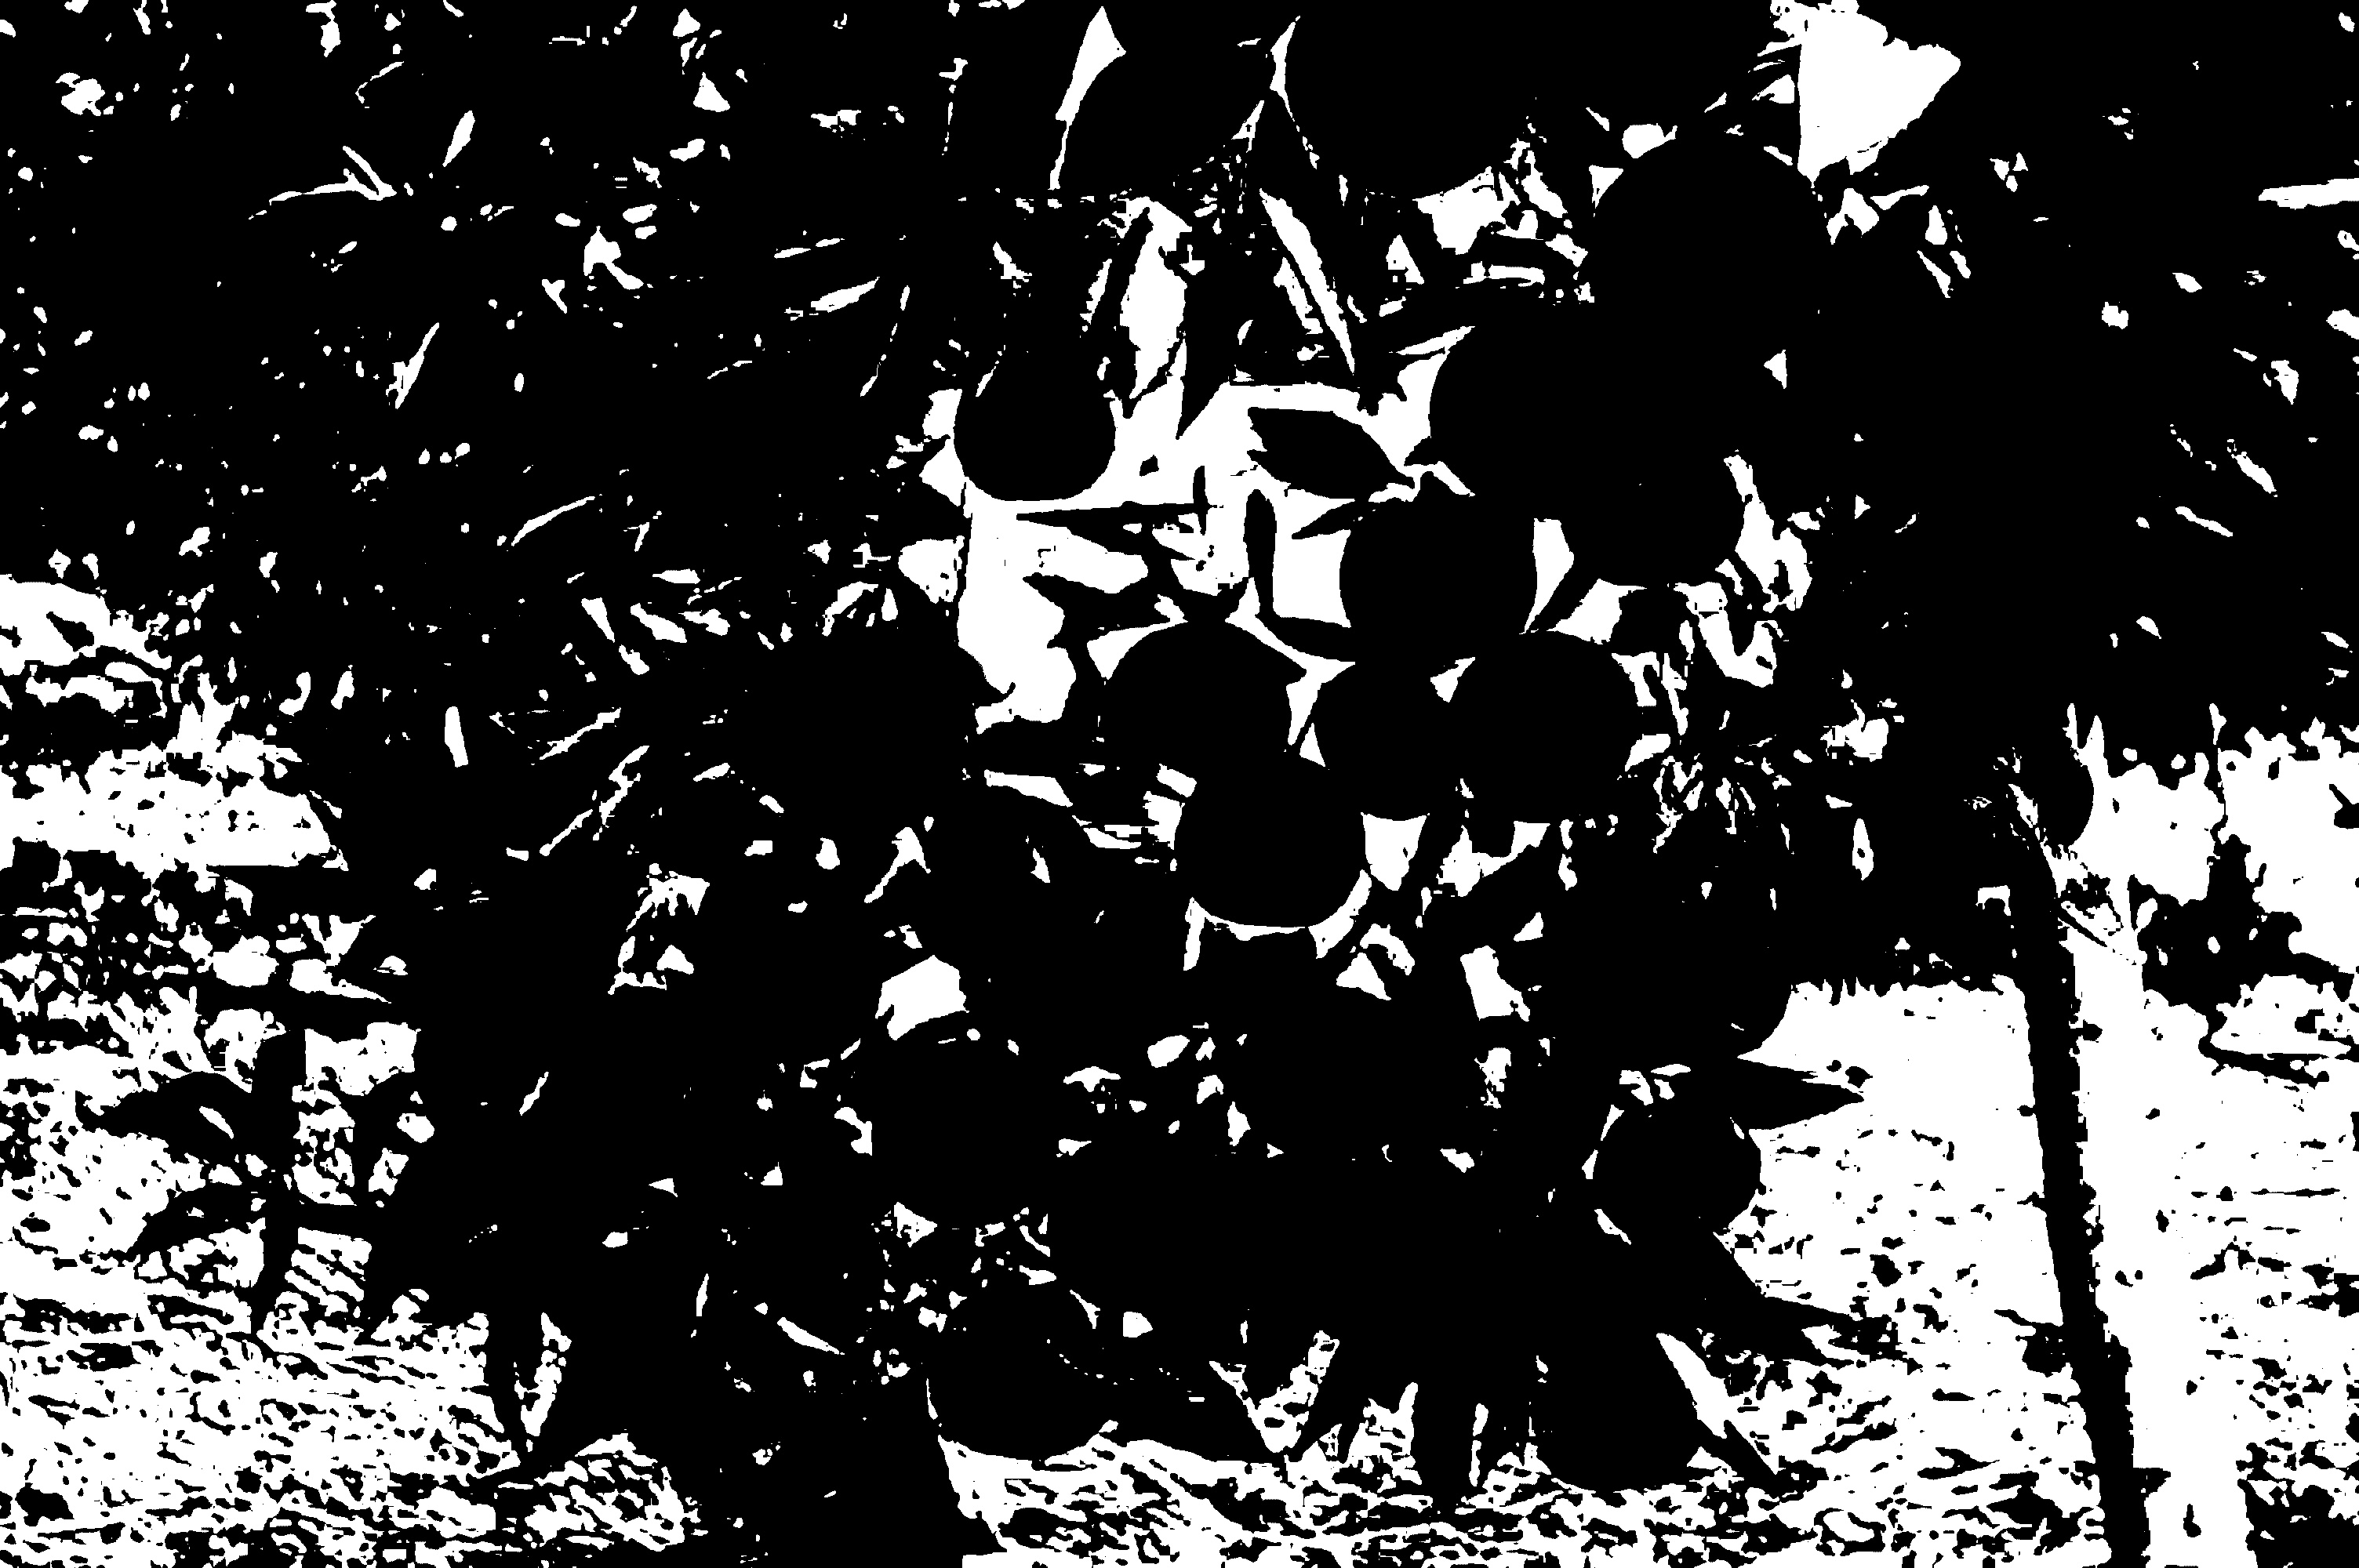
\includegraphics[width=\linewidth]{citrus1/citrus1_cb.jpg}\hfill
     	\caption{Result of step 4}
  \end{subfigure}
  \begin{subfigure}{.33\linewidth}
  	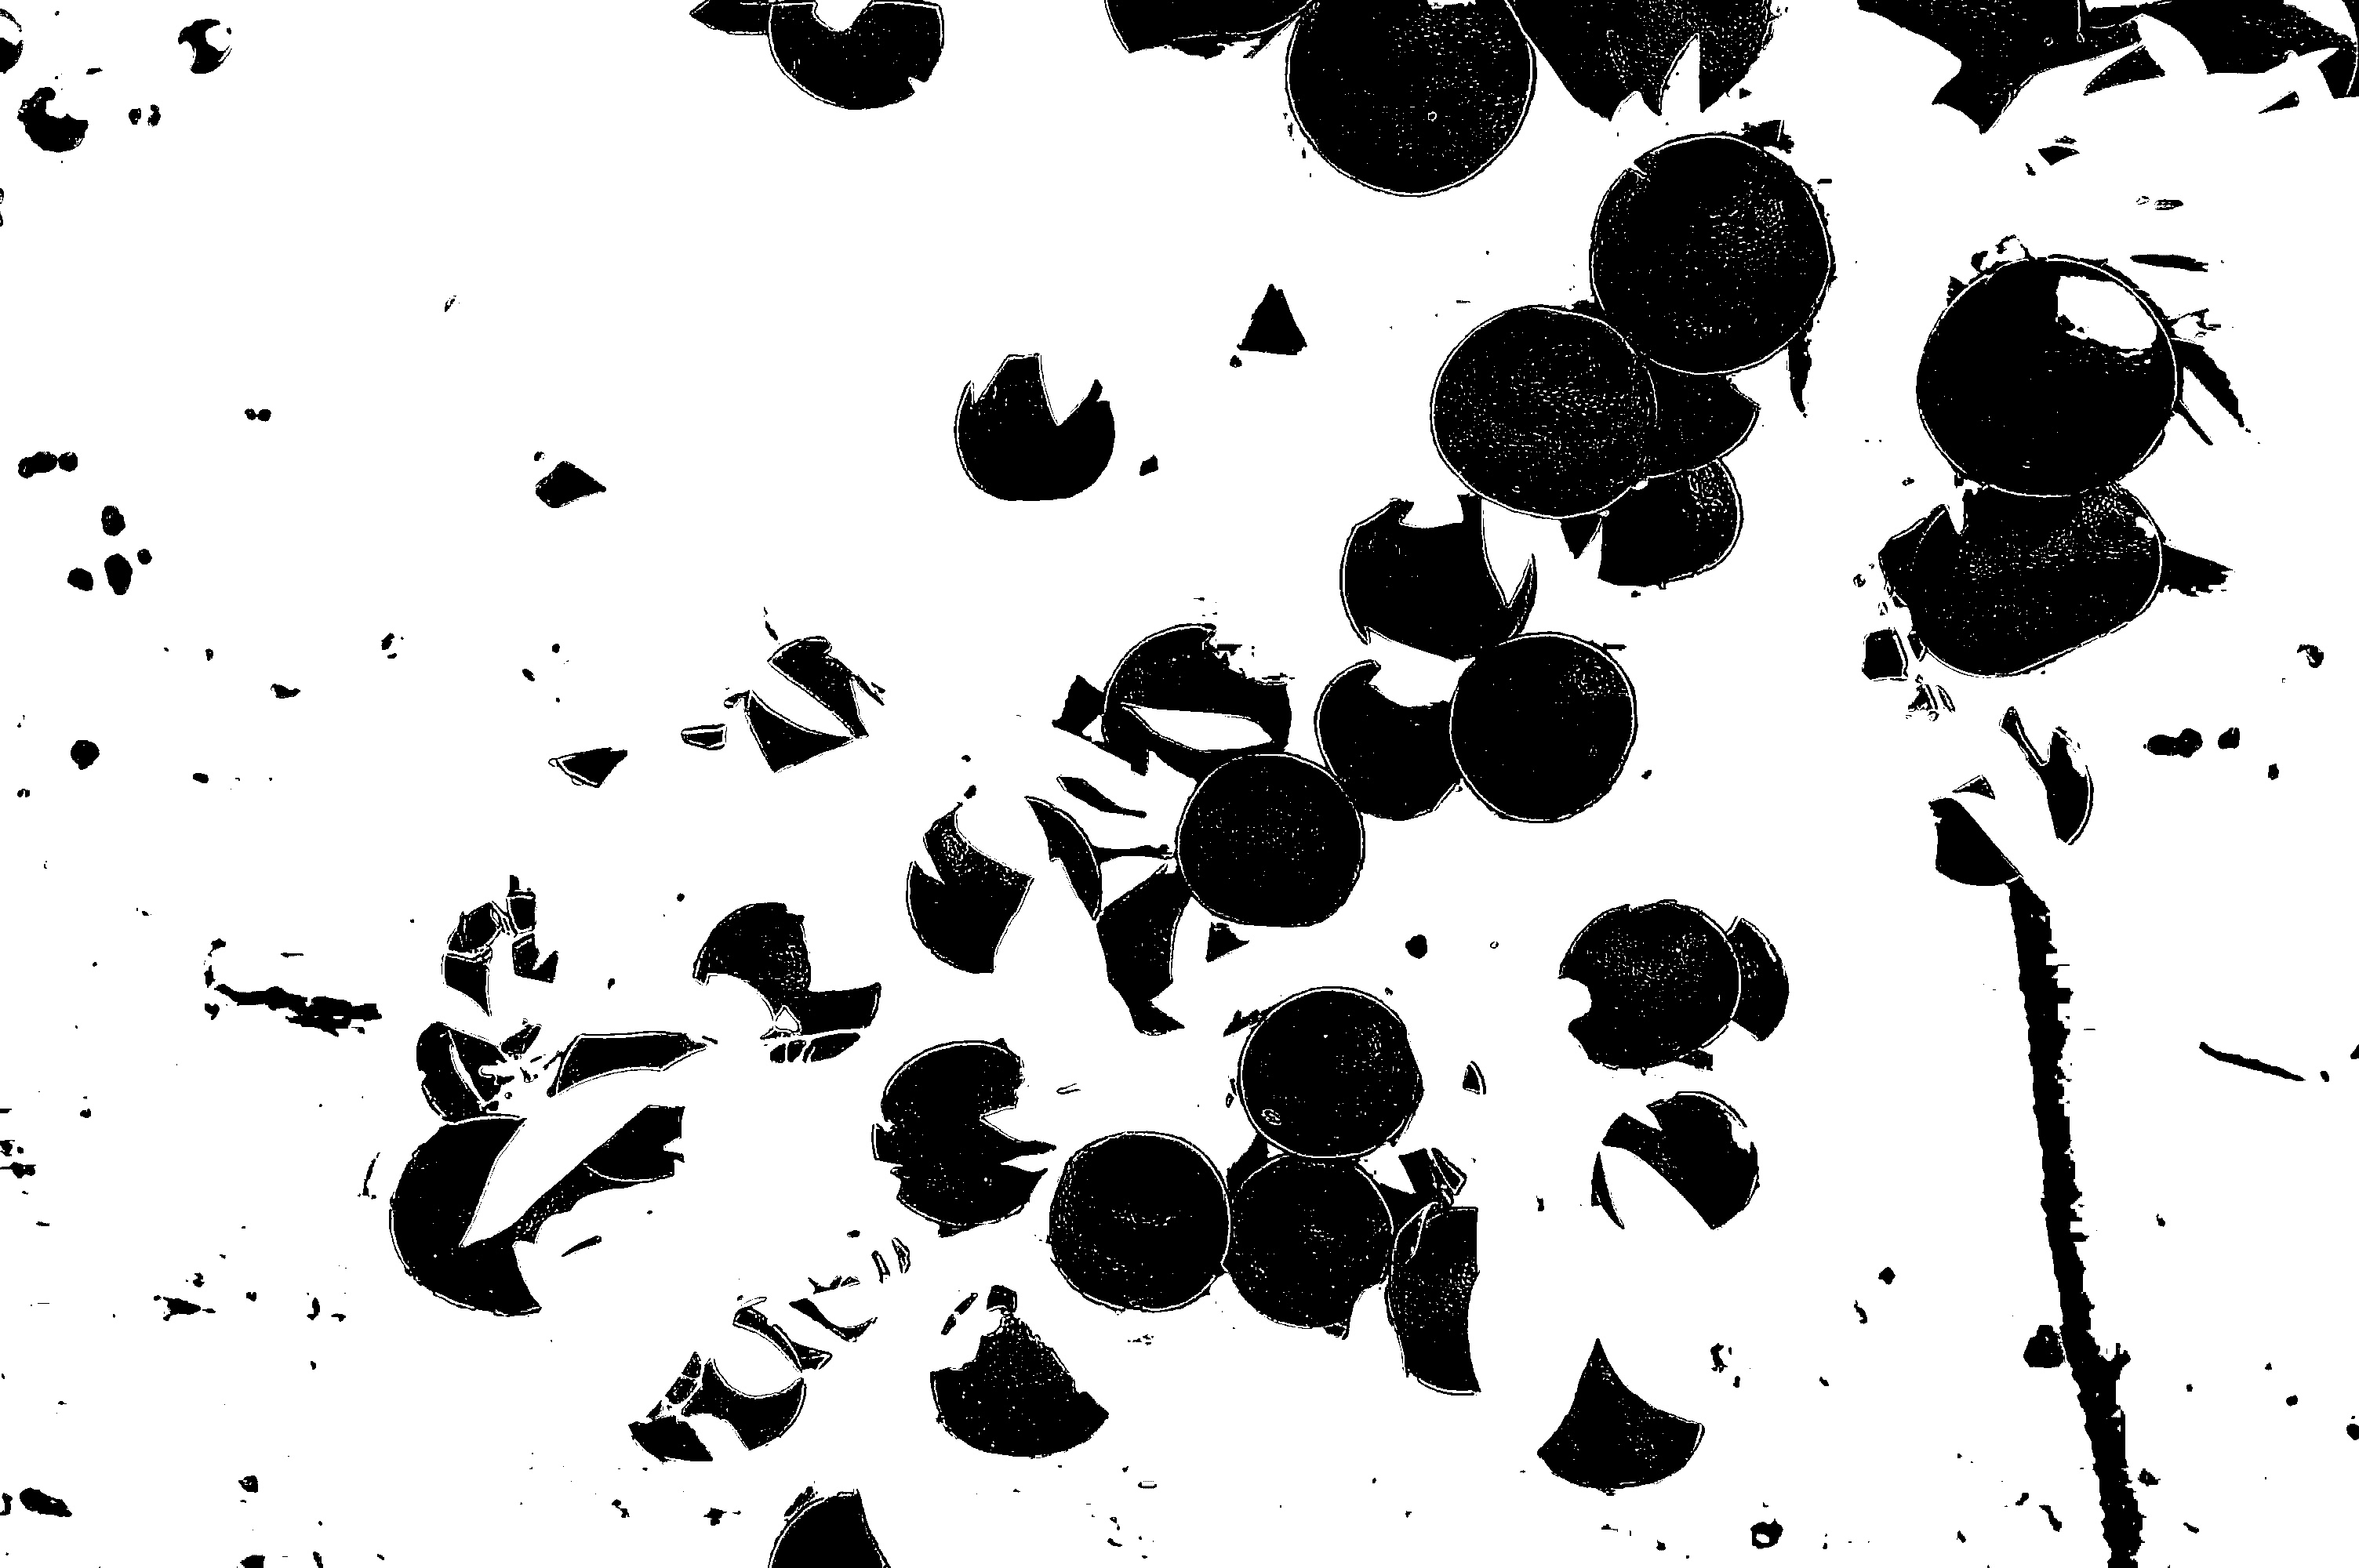
\includegraphics[width=\linewidth]{citrus1/citrus1_mask.jpg}
  	\caption{Result of step 5}
  \end{subfigure}\par\medskip
  \begin{subfigure}{.5\linewidth}
  	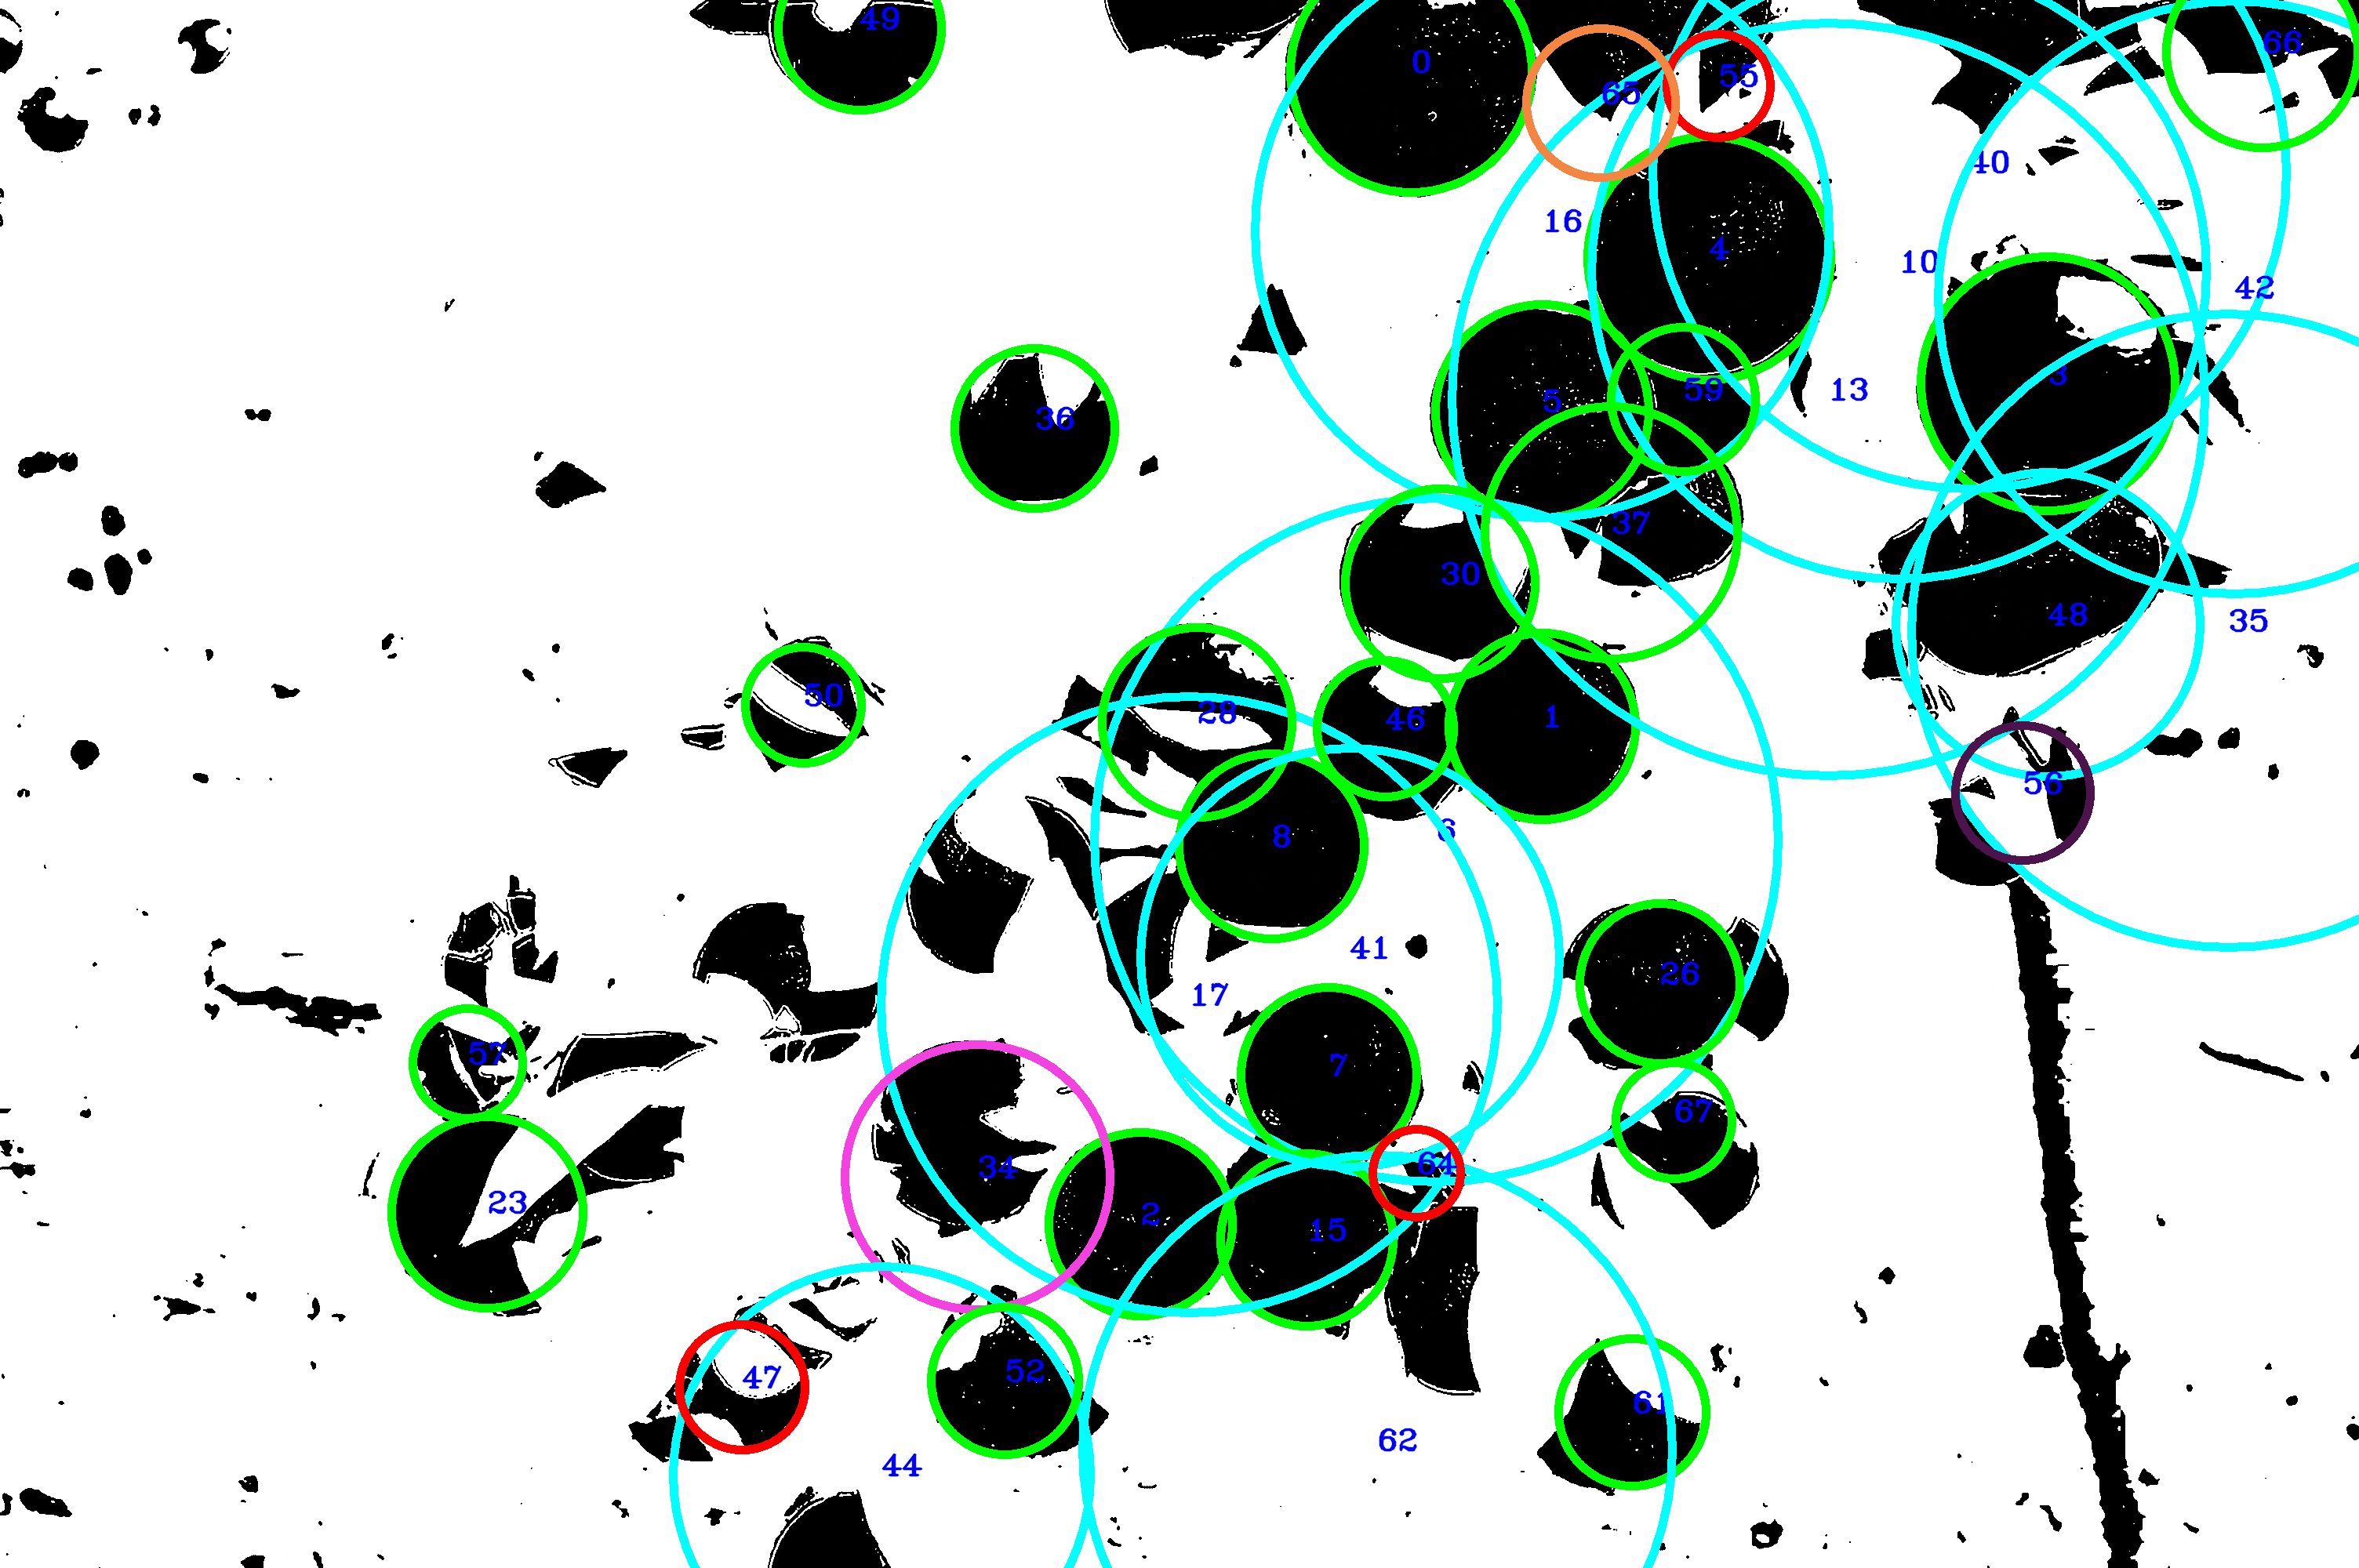
\includegraphics[width=\linewidth]{citrus1/citrus1_circles_mask.png}\hfill
	   	\caption{Result of step 6a}
  \end{subfigure}
  \begin{subfigure}{.5\linewidth}
  	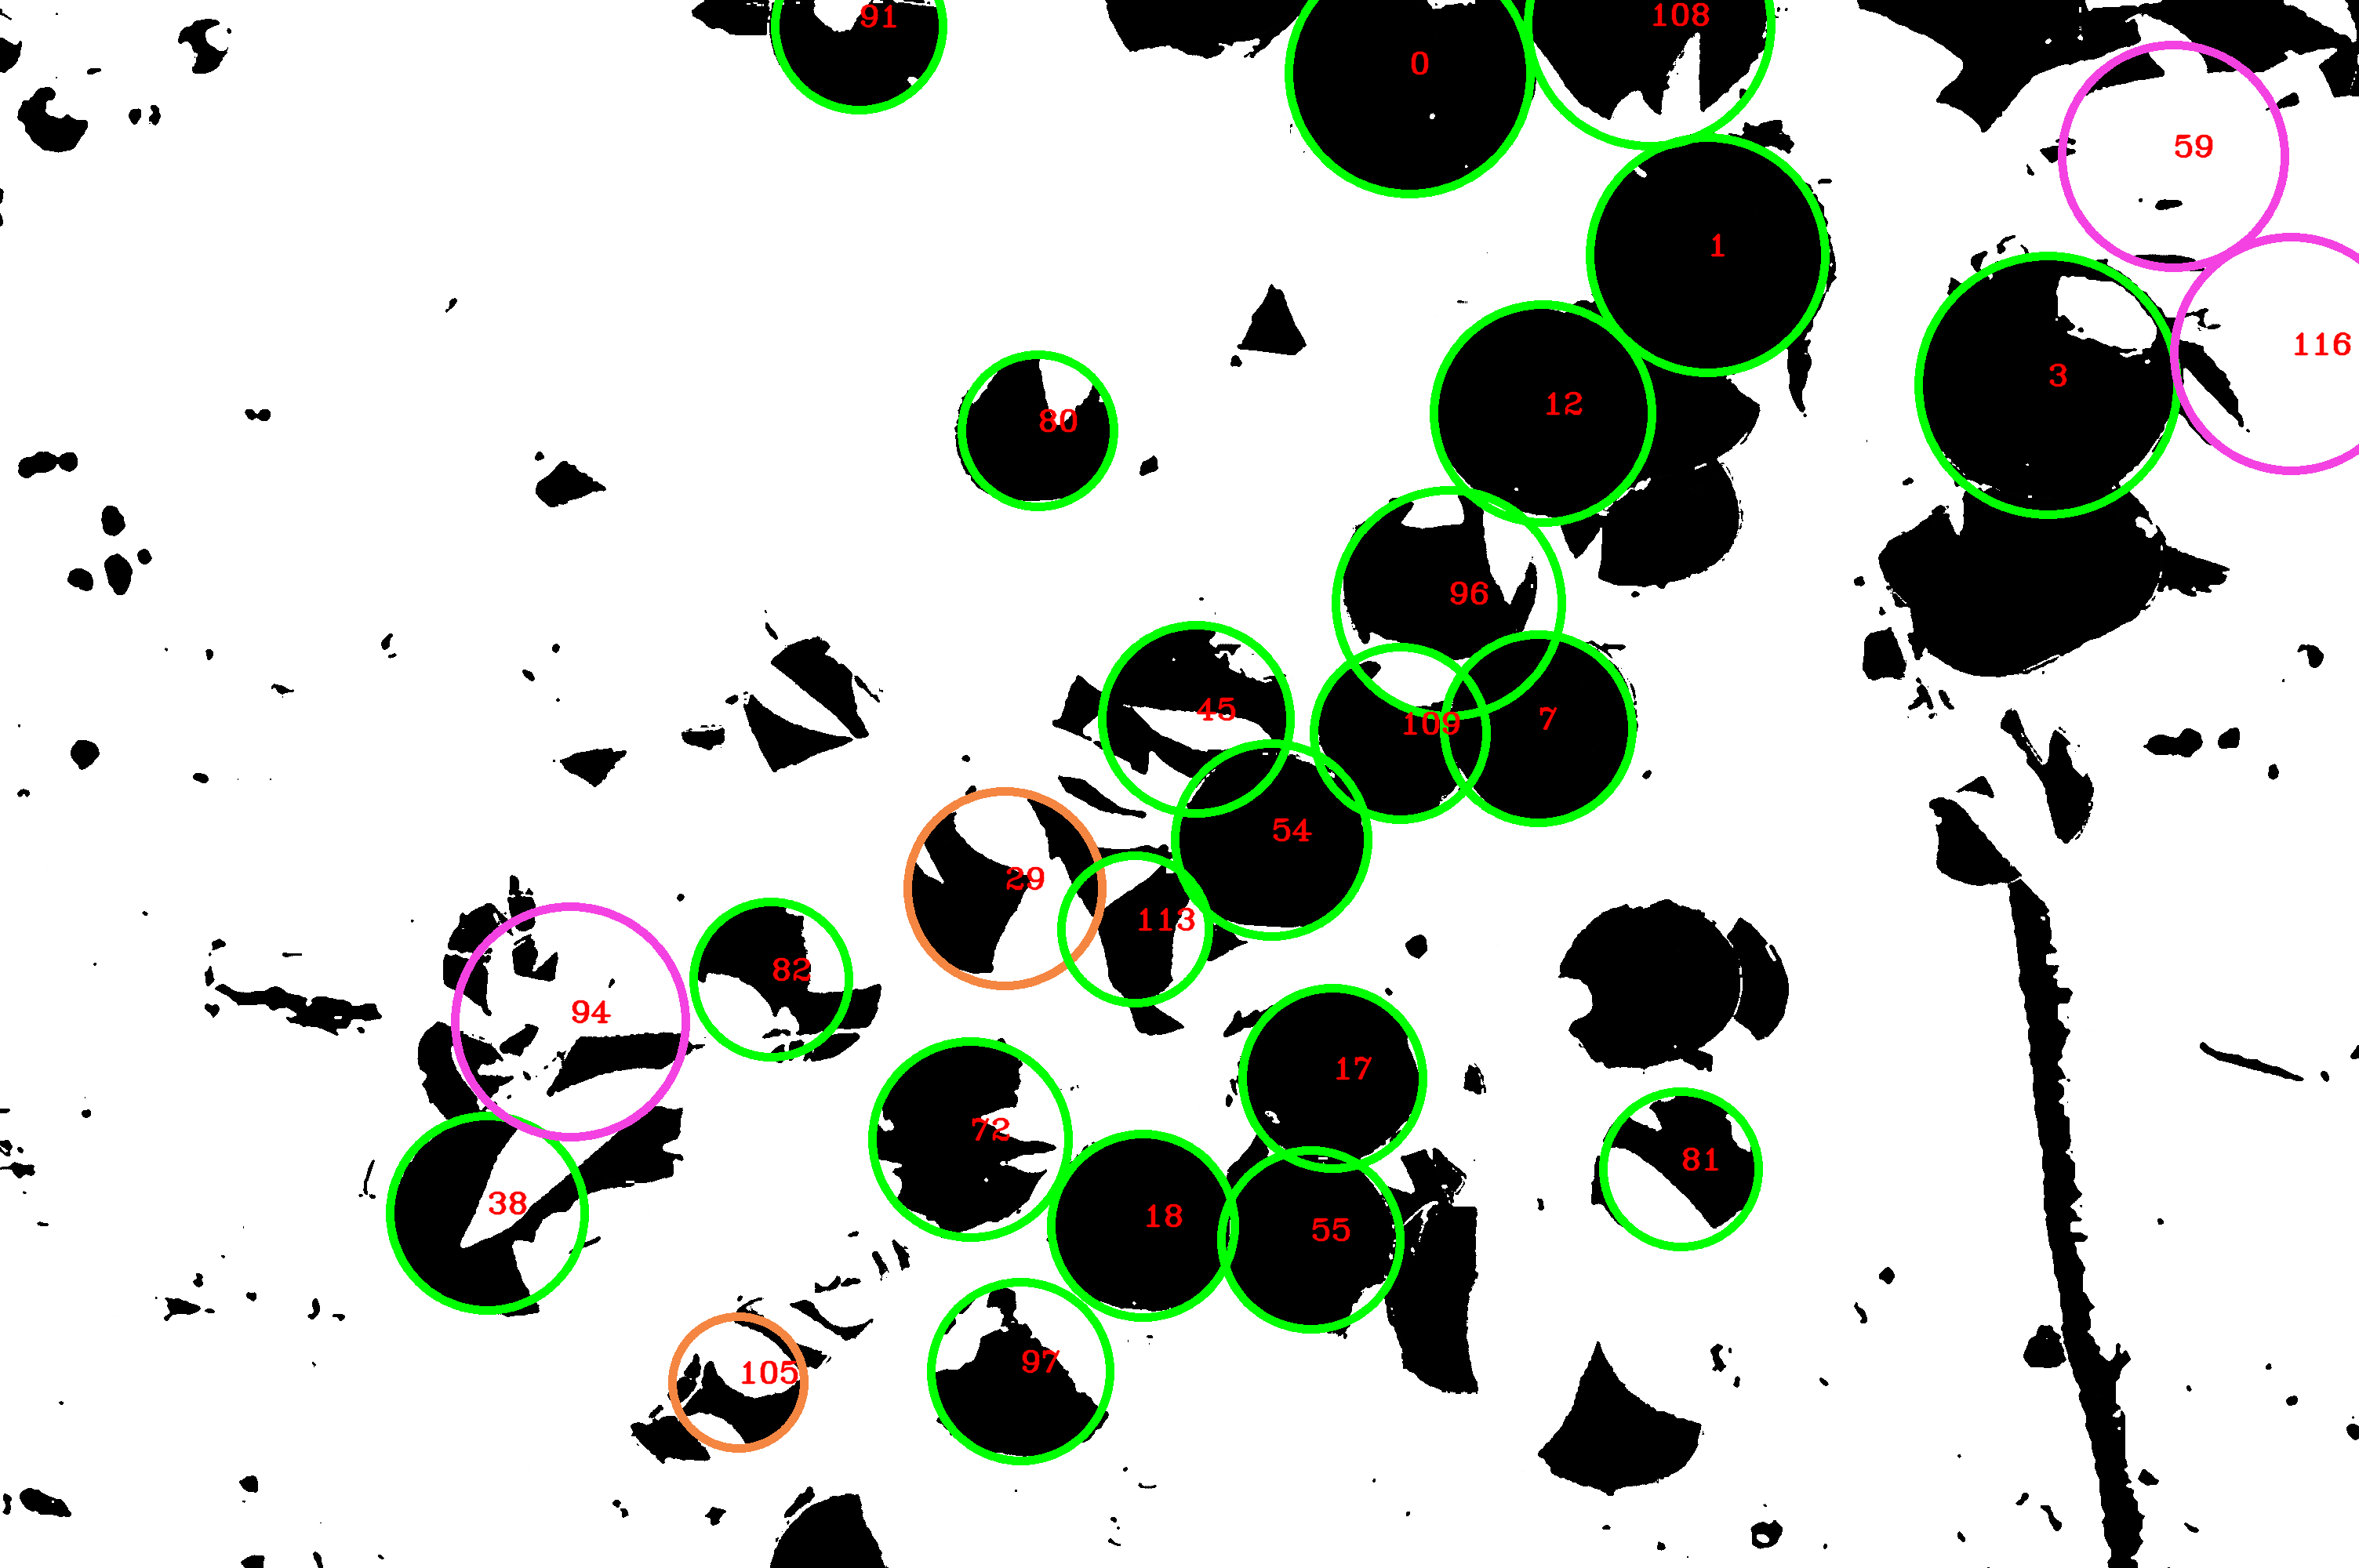
\includegraphics[width=\linewidth]{citrus1/citrus1_circles.png}\hfill
 	 \caption{Result of step 6b}
  \end{subfigure}
  \caption{An example image going through each step to detect the oranges within the image }
\end{figure*}


\section{Discussion}

\subsection{Limitations}

When we were testing our algorithm we noticed that it worked significantly better on images larger than 1300x1300px. It also does not work on images where the diameter of the oranges is greater than half of the screen size, or if the oranges are very small (less then 150px). We determined that this short coming can be easily overcome by using image resolutions above that size. In the application where this algorithm would be used the image quality would be known and the zoom of the image would be consistent allowing the mentioned shortcomings to be overcame. 



\bibliographystyle{ieeetr}
\bibliography{reference}





\vspace{12pt}

\end{document}
